\documentclass[tikz,border=7pt]{standalone}
\usepackage{palatino}
\usepackage{xcolor}
\usetikzlibrary{arrows.meta,calc}

\definecolor{mapink}{HTML}{20252B}
\definecolor{mapgray}{HTML}{707780}
\definecolor{mapline}{HTML}{9199A1}
\definecolor{mapblue}{HTML}{0072B2}
\definecolor{mapbluefill}{HTML}{F2F8FC}

\begin{document}
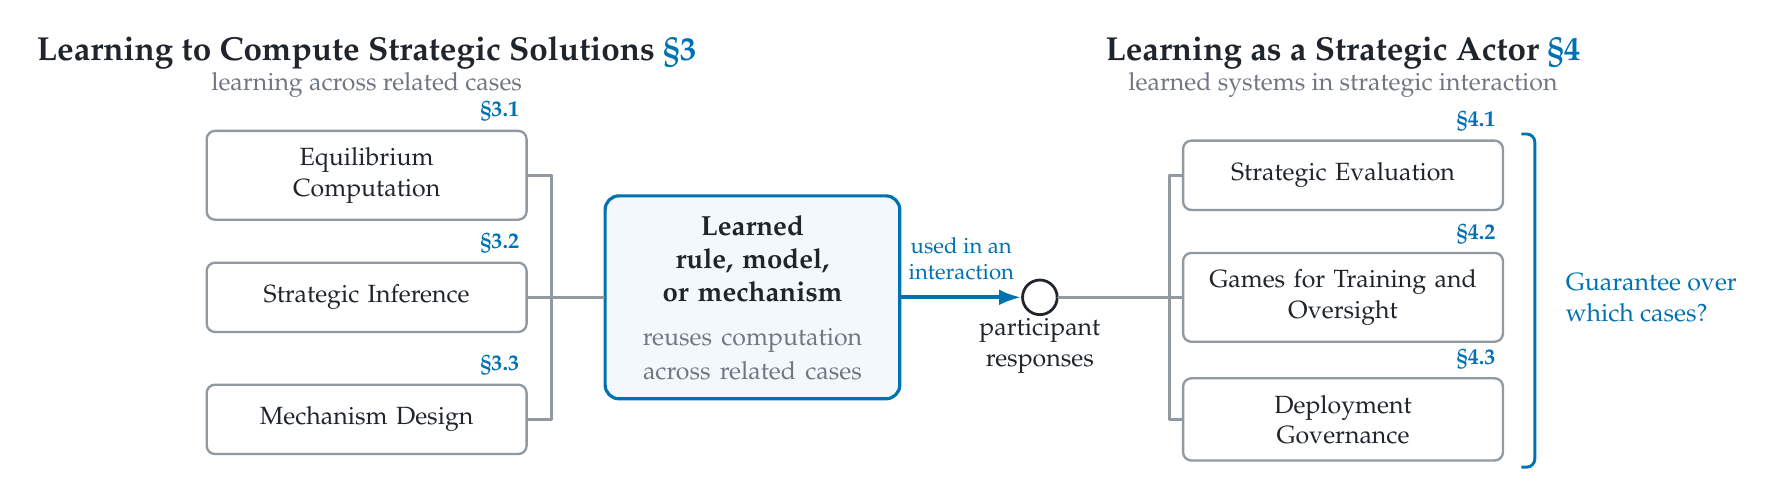
\begin{tikzpicture}[
  font=\rmfamily,
  domaincard/.style={
    draw=mapline,
    fill=white,
    text=mapink,
    line width=0.85pt,
    rounded corners=3pt,
    align=center,
    font=\rmfamily\small,
    text width=3.50cm,
    minimum width=3.90cm,
    minimum height=0.88cm,
    inner xsep=8pt,
    inner ysep=6pt
  },
  sectionref/.style={
    font=\rmfamily\bfseries\footnotesize,
    text=mapblue,
    fill=white,
    inner sep=1.5pt
  },
  learned/.style={
    draw=mapblue,
    fill=mapbluefill,
    text=mapink,
    line width=1.15pt,
    rounded corners=5pt,
    align=center,
    text width=3.25cm,
    minimum width=3.65cm,
    minimum height=1.68cm,
    inner sep=7pt
  },
  response/.style={
    circle,
    draw=mapink,
    fill=white,
    line width=1.0pt,
    minimum size=0.44cm,
    inner sep=0pt
  },
  branch/.style={
    draw=mapline,
    line width=1.15pt,
    line cap=round,
    line join=round
  },
  flow/.style={
    draw=mapblue,
    line width=1.35pt,
    -{Latex[length=2.8mm,width=2.0mm]},
    line cap=round
  }
]

\node[font=\rmfamily\bfseries\large,text=mapink] at (-5.50,3.10)
  {Learning to Compute Strategic Solutions \textcolor{mapblue}{\S 3}};
\node[font=\rmfamily\small,text=mapgray] at (-5.50,2.70)
  {learning across related cases};
\node[font=\rmfamily\bfseries\large,text=mapink] at (6.90,3.10)
  {Learning as a Strategic Actor \textcolor{mapblue}{\S 4}};
\node[font=\rmfamily\small,text=mapgray] at (6.90,2.70)
  {learned systems in strategic interaction};

\node[domaincard] (eq) at (-5.50,1.55) {Equilibrium Computation};
\node[sectionref,anchor=south east] at ($(eq.north east)+(-0.05,0.04)$) {\S 3.1};
\node[domaincard] (inf) at (-5.50,0) {Strategic Inference};
\node[sectionref,anchor=south east] at ($(inf.north east)+(-0.05,0.04)$) {\S 3.2};
\node[domaincard] (md) at (-5.50,-1.55) {Mechanism Design};
\node[sectionref,anchor=south east] at ($(md.north east)+(-0.05,0.04)$) {\S 3.3};

\node[domaincard] (eval) at (6.90,1.55) {Strategic Evaluation};
\node[sectionref,anchor=south east] at ($(eval.north east)+(-0.05,0.04)$) {\S 4.1};
\node[domaincard] (games) at (6.90,0) {Games for Training and\\Oversight};
\node[sectionref,anchor=south east] at ($(games.north east)+(-0.05,0.04)$) {\S 4.2};
\node[domaincard] (gov) at (6.90,-1.55) {Deployment Governance};
\node[sectionref,anchor=south east] at ($(gov.north east)+(-0.05,0.04)$) {\S 4.3};

\node[learned] (object) at (-0.60,0) {
  {\bfseries Learned rule, model,\\or mechanism}\\[5pt]
  {\small\color{mapgray}reuses computation\\across related cases}
};
\node[response] (responses) at (3.05,0) {};

\coordinate (leftspine) at (-3.15,0);
\draw[branch] (eq.east) -- (-3.15,1.55);
\draw[branch] (inf.east) -- (leftspine);
\draw[branch] (md.east) -- (-3.15,-1.55);
\draw[branch] (-3.15,1.55) -- (-3.15,-1.55);
\draw[branch] (leftspine) -- (object.west);

\draw[flow] (object.east) -- (responses.west);
\node[font=\rmfamily\footnotesize,text=mapblue,fill=white,inner sep=1.5pt,align=center]
  at ($(object.east)!0.50!(responses.west)+(0,0.49)$)
  {used in an\\interaction};
\node[font=\rmfamily\small,text=mapink,align=center] at (3.05,-0.62)
  {participant\\responses};

\coordinate (rightspine) at (4.70,0);
\draw[branch] (responses.east) -- (rightspine);
\draw[branch] (4.70,1.55) -- (4.70,-1.55);
\draw[branch] (4.70,1.55) -- (eval.west);
\draw[branch] (rightspine) -- (games.west);
\draw[branch] (4.70,-1.55) -- (gov.west);

\draw[draw=mapblue,line width=1.05pt,rounded corners=3pt]
  ($(eval.north east)+(0.22,0.07)$) -- ++(0.17,0)
  -- ($(gov.south east)+(0.39,-0.07)$) -- ++(-0.17,0);
\node[font=\rmfamily\small,text=mapblue,align=left,anchor=west]
  at ($(games.east)+(0.66,0)$) {Guarantee over\\which cases?};

\end{tikzpicture}
\end{document}
